\documentclass[aspectratio=169,13pt,t] {beamer}
\mode<presentation>
{
  \usetheme{Madrid}
  \usecolortheme{beaver}
  \usefonttheme{serif}
  \setbeamertemplate{caption}[numbered]
  \setbeamertemplate{items}[default]
}

\usepackage[,UTF8,linespread=1.2]{ctex}
\usepackage{graphicx}
\usepackage{caption}
\captionsetup[figure]{name=图,labelsep=period}
\usepackage{tcolorbox}
\usepackage{xcolor}

\definecolor{xy_blue}{cmyk}{0.6,0.35,0.0,0.4}
\definecolor{xy_orange}{cmyk}{0.0,0.7,1.0,0.0}
\definecolor{xy_green}{cmyk}{0.2,0.0,1.0,0.15}
\xdefinecolor{xy_gold}{RGB}{135,103,79}

\setbeamercolor{section number projected}{fg=red,bg=red!20}
\setbeamercolor{item}{fg=xy_gold}

\usepackage{amsthm}
\newtheorem{question}{问题}
\newtheorem*{solve}{解:}
\newtheorem{exam}{例}

\newtcolorbox{summarybox}[1][]{
  colback=purple!10, colframe=purple!70!black,
  fonttitle=\bfseries, title=#1, arc=1mm,
  boxrule=0pt, drop shadow, left=2mm, right=2mm, top=2mm, bottom=2mm,
}

\AtBeginSection[]{
  \begin{frame}<beamer>
    \frametitle{本节主要内容}
    \tableofcontents[currentsection,currentsubsection]
  \end{frame}
}

\AtBeginDocument{
  \setlength{\abovedisplayskip}{3pt}
  \setlength{\belowdisplayskip}{3pt}
}

\title[3.1.1函数的概念（二）]{3.1.1函数的概念（二）}
\author[好好学习，努力向上]{}\institute{}\date{\today}
\begin{document}
\begin{frame}{}
  \titlepage
\end{frame}

\begin{frame}{内容概览}
  \tableofcontents
\end{frame}

\section{教材内容}

\begin{frame}{教材截图 1}
  \begin{figure}
    \centering
    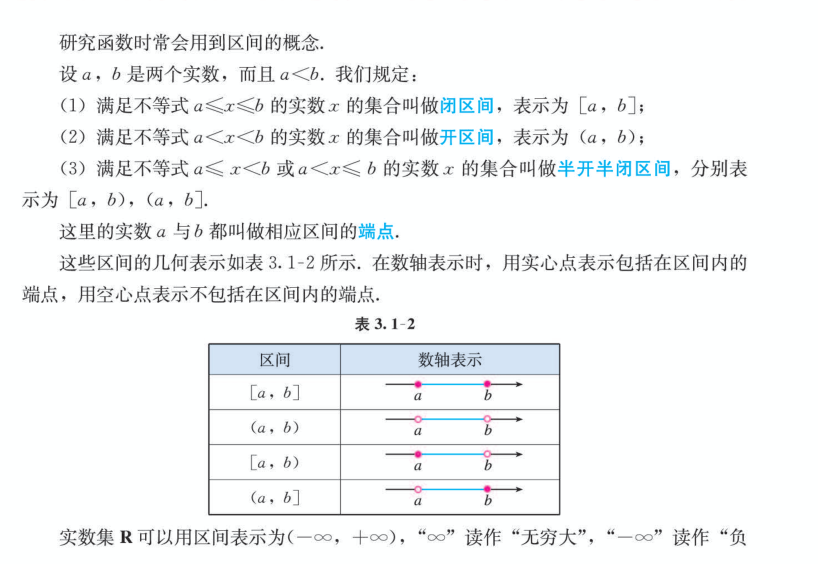
\includegraphics[scale=0.85]{Figures/屏幕截图 2026-10-12 195609.png}
  \end{figure}
\end{frame}

\begin{frame}{教材截图 2}
  \begin{figure}
    \centering
    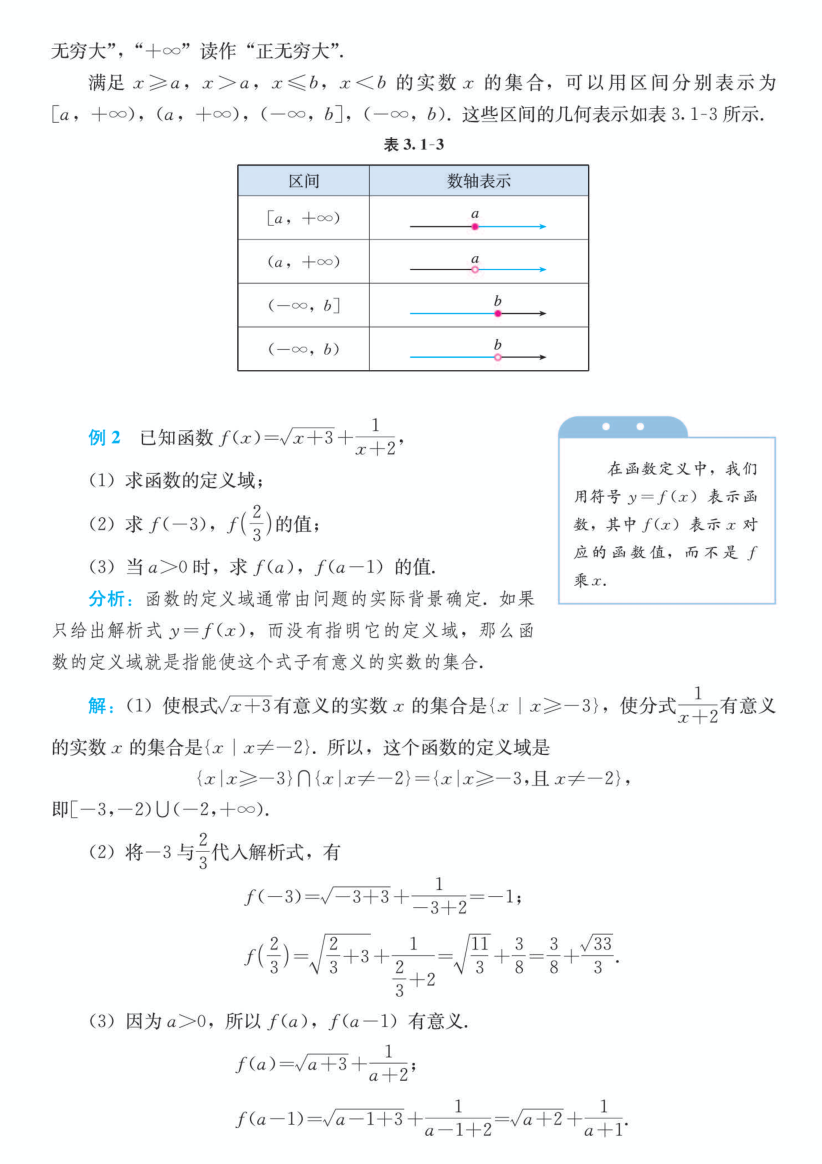
\includegraphics[scale=0.85]{Figures/屏幕截图 2026-10-12 195624.png}
  \end{figure}
\end{frame}

\begin{frame}{教材截图 3}
  \begin{figure}
    \centering
    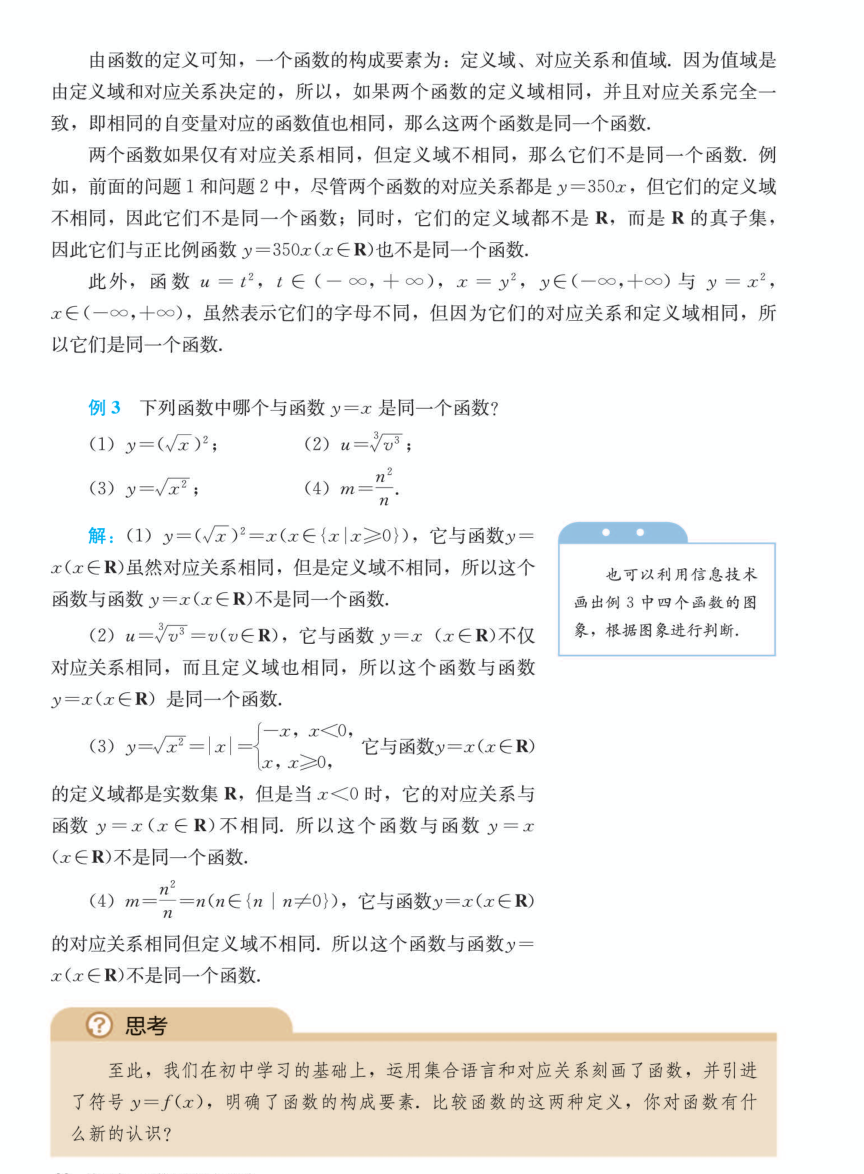
\includegraphics[scale=0.85]{Figures/屏幕截图 2026-10-12 195638.png}
  \end{figure}
\end{frame}

\begin{frame}{教材截图 4}
  \begin{figure}
    \centering
    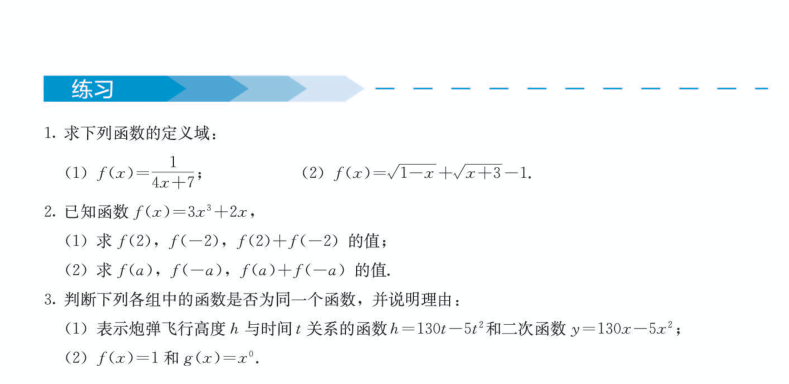
\includegraphics[scale=0.85]{Figures/屏幕截图 2026-10-12 195646.png}
  \end{figure}
\end{frame}

\end{document}